\documentclass{article}

\usepackage{amsmath}
\usepackage{bm}
\usepackage{graphicx}


\title{Prosjektoppgave 2}
\author{Edvart Bjerke}
\date{October 2024}
\begin{document}
\graphicspath{ {./images/} }
\maketitle

\section{Bildesegmentering}
I denne oppgaven skal bilder segmenteres ved å klassifisere individuelle pixler.
Det er valgt å bruke en maximum-likelihood metode, med antatt normalfordelte egenskaper.
Som foreslått av oppgaven brukes den følgende transformasjonen til å definere egenskapene
til en gitt pixel:

\[\bm{x} = [t_1, t_2]^t\]
\[t_1 = \frac{R}{R+G+B}, \quad t_2 = \frac{G}{R+G+B}\]

Hvor $R$, $G$ og $B$ er hendholdsvis den røde, grønne og blå fargeverdien til pixelet.
Siden den blå kanalen er med i normaliseringen (intensiteten $R+G+B$) får vi med oss all fargeinformasjon
i egenskapsvektoren $x$ med to parametre.

\newpage
\section{Utprøving av klassifikatoren}
For å teste om klassifikatoren fungerer brukes følgende bilde:

\begin{figure}[h]
    \centering
    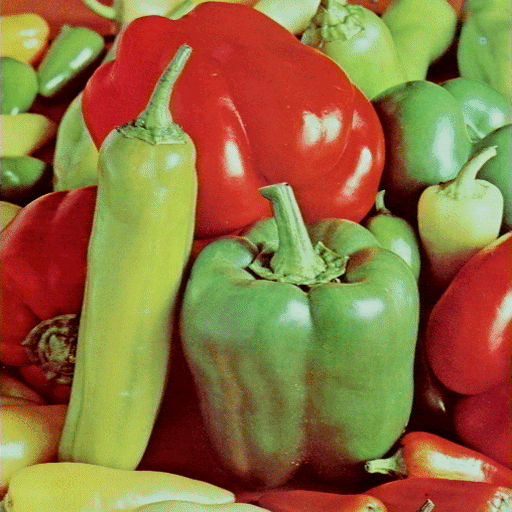
\includegraphics[width=4.7cm]{Bilde1}
    \caption{Testbilde}
\end{figure}

For å trene opp klassifikatoren må det produseres et datasett av labelede sampler (pixler).
For å gjøre dette enkelt, velges det ut regioner som kun inneholder pixler av èn av klassene.

Følgende klasser er valgt for denne mønstergjenkjenningsoppgaven:
\begin{itemize}
    \item[ ] $\omega_1$: Rød paprika
    \item[ ] $\omega_2$: Grønn paprika
    \item[ ] $\omega_3$: Chili
\end{itemize}

Dette er altså et klassifiseringsproblem med 3 klasser. Det velges ut tre regioner,
og pixlene innenfor disse danner treningssettet som brukes til å finne vektene i max-likelihood diskriminantfunksjonene.

Figur 2 viser regionene (valgt manuelt):
\begin{figure}[h]
    \centering
    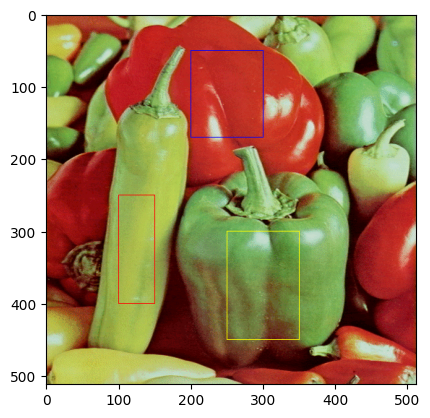
\includegraphics[width=4.84cm]{test_regions}
    \caption{Regioner for treningssettet}
\end{figure}

Pixelverdiene innenfor regionene tildeles labeler (klasse-index 1-3), og 
verdiene transformeres til egenskapsrommet definert tidligere. Det settes opp en datamatrise
som inneholder alle sampler i egenskapsrommet, med følgende form:
$$
\begin{bmatrix}
    {}^1\omega & {}^1\pmb{x}^t\\
    \vdots & \vdots \\
    {}^n\omega & {}^n\pmb{x}^t
\end{bmatrix}
=
\begin{bmatrix}
    {}^1\omega & {}^1t_1 & {}^1t_{2}\\
    \vdots & \vdots & \vdots \\
    {}^n\omega & {}^nt_1 & {}^nt_{2}
\end{bmatrix}
$$
Slik at hver rad $i$ inneholder klassetilhørligheten (${}^i\omega$) og egenskapsvektoren (${}^i\pmb{x}^t$) til pixel $i$ i treningssettet.
Dette formatet er kompatibelt med implementasjonen av klassifikatorene fra prosjektoppgave 1.

\subsection*{Beslutningsregel og diskriminantfunksjoner}
For denne oppgaven brukes maximum-likelihood metoden som grunnlag for beslutninsregelen.
Ved hjelp av diskriminantfunksjoner kan denne beslutningsregelen formuleres som følger:

\[ \text{Velg klasse } \omega_m \text{ dersom } g_m(\pmb{x}) \geq g_i(\pmb{x}) \quad i = 1,..., c\]
    Hvor diskriminantfunksjonen $g_i(\pmb{x})$ er gitt ved:
\[ g_i(\pmb{x}) = \pmb{x}^tW_i\pmb{x} + {\pmb{w}_i}^t\pmb{x} + w_{i0}\]
der
\[W_i = -\frac{1}{2}\hat{\Sigma}^{-1}\]
\[\pmb{w}_i = \hat{\Sigma}^{-1} \hat{\pmb{\mu}}_i\]
\[w_{i0} = -\frac{1}{2}{\hat{\pmb{\mu}}_i}^t\hat{\Sigma}^{-1}\hat{\pmb{\mu}}_i -\frac{1}{2} \ln{|\hat{\Sigma}_i|} + \ln{P(\omega_i)}\]

$\hat{\pmb{\mu}}_i$ og $\hat{\Sigma}$ er estimatene for det antatte normalfordelte egenskapsrommet. Disse estimeres hendholdsvis av 
sampel-middelet og sampel-variansen. A priori sannsynlighetene $P(\omega_i)$ estimeres også, basert på størrelsene av regionene.
I psuedo-kode ser metodikken slik ut:
\begin{verbatim}
img_test = load(img_test)
pixels_w_1 = img[region_1]
pixels_w_2 = img[region_2]
pixels_w_3 = img[region_3]

training_set = create_matrix(pixels_w_1, pixels_w_2, pixels_w_3)
for each i = 1, ..., 3:
    P_i = compute_a_priori(training_set, class=i)
    sigma_i = compute_sample_mean(training_set, class=i)
    mu_i = compute_sample_variance(training_set, class=i)
    W_i = get_W_matrix(sigma_i)
    w_i = get_w_vector(sigma_i, mu_i)
    w_i_0 = get_w0(sigma_i, mu_1, P_i)
\end{verbatim}

\newpage
\subsection*{Plotting av egenskapsrommet}
For å visualisere fordelingen av egenskaper for de forskjellige samplene kan vi plotte
treningsdataen. Dette gir en indikasjon på om vi har god separasjon mellom klasser og om klassifikatoren
bør kunne skille mellom de.

\begin{figure}[h]
    \centering
    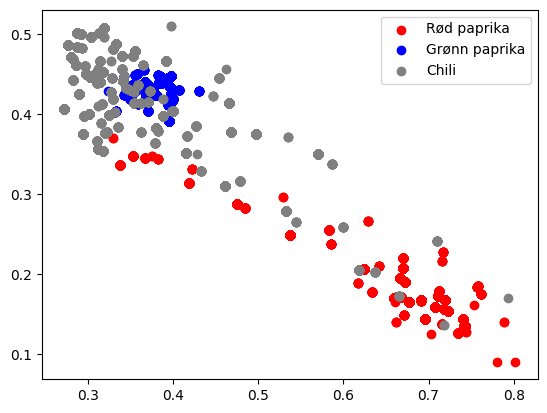
\includegraphics[width=4.84cm]{plott_paprika}
    \caption{Plott av treningsdata i det to-dimensjonale egenskapsrommet}
\end{figure}

Fra denne figuren ser vi at det er nokså god separasjon mellom rød og grønn paprika, men at dataen for chili 
innblandes noe. Vi bør altså kunne forvente at klassifikatoren ikke bør klassifisere rød paprika som grønn paprika, eller omvendt.
Samtidig bør vi forvente at det blir vanskelig å separere ut chili.

\subsection*{Resultater, prøvebilde}
Ved bruk av vektene som er trent opp fra datasettet, gjør vi en klassifisering av hvert enkelt pixel.
Resultatet av klassifiseringen for et gitt pixel blir brukt til å fargelegge et tomt bilde, slik at vi kan visualisere
segmenteringen. Gangen er som følger:
\begin{verbatim}
result_img = empty_image(size(test_image))
for each coordinate in test_image:
    # Extract the pixel and transform to feature space
    pixel_value = test_image[coordinate]
    x = transform(pixel_value)   

    # Apply the decision rule
    predicted_class = argmax(g_1(x), g_2(x), g_3(x))
    
    # Visualize the classification
    result_img[coordinate] = highlight_color(predicted_class)

\end{verbatim}
Resultatet av klassifiseringen er vist i figuren under:
\newpage
\begin{figure}[h]
    \centering
    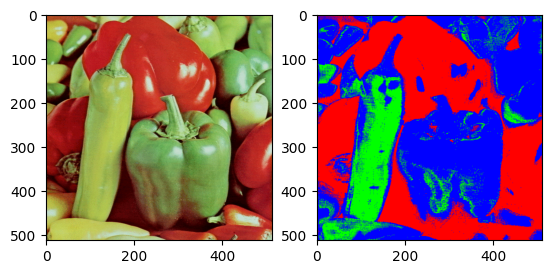
\includegraphics[width=10cm]{resultat_paprika}
    \caption{Resultatet av klassifiseringen, vist ved siden av det originale prøvebildet. Fargene representerer klassifiseringen: Rød paprika (rødt), grønn paprika (blått) og chili (grønt)}
\end{figure}
Vi ser altså at klassifikatoren gjør en grei jobb på å skille mellom klassene.
Det er også tydelig at chili forveksles med de andre klassene, mens rød og grønn paprika sjeldent blir forvekslet med hverandre.
Dette stemmer overens med separabiliteten av distribusjonene sett i plottet over.

\subsection*{Resultater, perm}
Nøyaktig samme fremgangsmåte er brukt her for å klassifisere rød/blå perm mot bakgrunn.
Den eneste forskjellen er at vi bruker et eget testbilde for å evaluere klassifikatoren.

\begin{figure}[h]
    \centering
    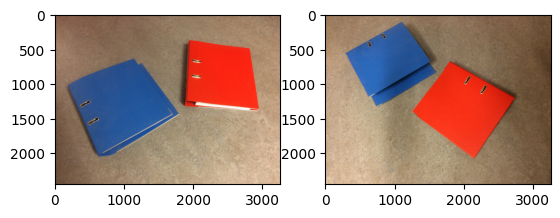
\includegraphics[width=10cm]{permer}
    \caption{Treningsbilde (venstre) og testbilde (høyre)}
\end{figure}

Regioner velges ut manuelt, pixler trekkes ut og de transformerte samplene brukes
til å trene opp vektene i klassifikatoren (diskriminantfunksjonene).
\newpage
\begin{figure}[h]
    \centering
    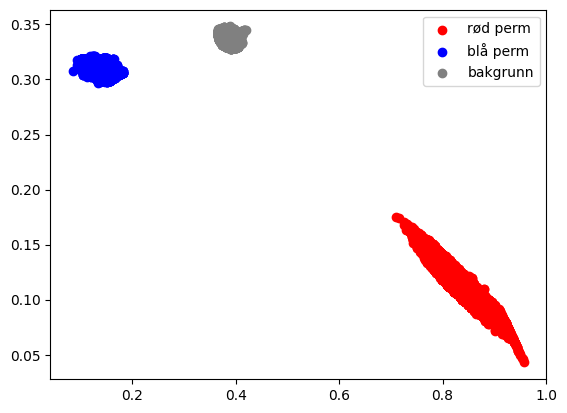
\includegraphics[width=7cm]{egenskap_perm}
    \caption{Plott av treningsdata i egenskapsrommet}
\end{figure}

Plottet viser svært god separasjon mellom klassene i egenskapsrommet. 
For dette problemet bør vi kunne oppnå veldig lave feilrater selv med en primitivv klassifikator.

\begin{figure}[h]
    \centering
    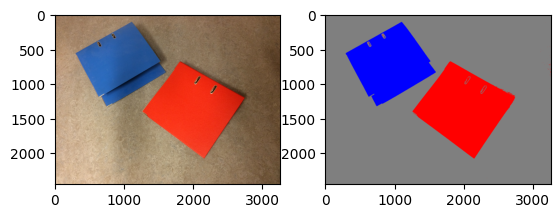
\includegraphics[width=7cm]{resultat_perm.png}
    \caption{Testbilde (venstre) og resultat av klassifisering (høyre)}
\end{figure}

Resultatene viser svært god klassifisering. Dette kommer av at vi har 
lav varians i fargeverdiene til pixlene av de forskjellige klassene.

\newpage
\subsection*{Resultater, egne bilder}
Til slutt er det forsøkt å segmentere bilde inn i `nødutgang`, `brannalarm` og `bakgrunn`.
\begin{figure}[h]
    \centering
    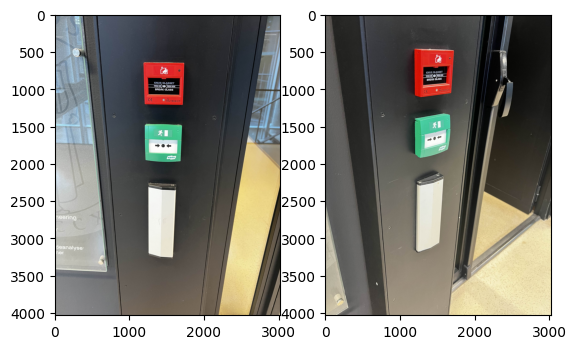
\includegraphics[width=7cm]{egne}
    \caption{Treningsbilde (venstre) testbilde (høyre)}
\end{figure}
\begin{figure}[h]
    \centering
    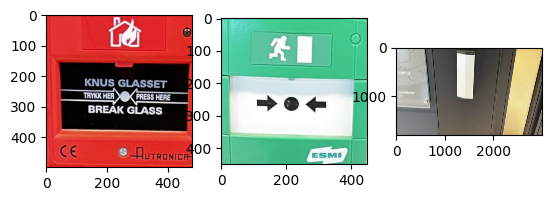
\includegraphics[width=7cm]{egne_regioner}
    \caption{Regioner brukt til treningssettet}
\end{figure}
\begin{figure}[h!]
    \centering
    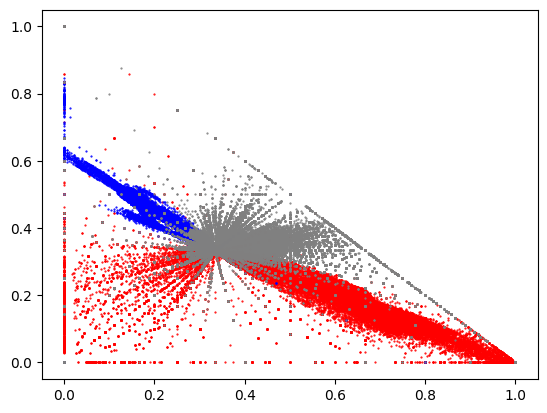
\includegraphics[width=7cm]{egne_egenskapsrom}
    \caption{Plott av egenskapsrom for treningssettet}
\end{figure}

\newpage
Figur 10 viser at treningssettet er komplisert, og det vil være
vanskelig å bestemme gode desisjonsregioner, da de forskjellige klassene
inneholder noe av de samme fargene. Likevel, klarer vi å oppnå greie resultater i segmenteringen
med våre enkle diskriminantfunksjoner:

\begin{figure}[h!]
    \centering
    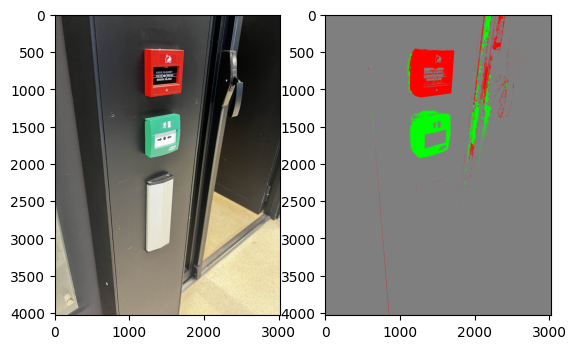
\includegraphics[width=10cm]{egne_resultater.png}
    \caption{Resultat av max-likelihood segmentering}
\end{figure}

Vi får naturligvis en del feilklassifiseringer, spesielt for bakgrunnen.
Vi ser også at den hvite delen av nødutgangbryteren (og den sorte delen av brannalarmen) forvirres med bakgrunn.
Det kan se ut som at å kun se på fargeinformasjon for individuelle pixler ikke er tilstrekkelig for å 
klassifisere disse objektene godt. Her må man nok dra inn flere egenskaper og bruke en mer sofistikert beslutningsregel. 
Man må nok også se på større områder om gangen, i stedet for å vurdere èn og èn pixel individuelt.


\end{document}